% Options for packages loaded elsewhere
\PassOptionsToPackage{unicode}{hyperref}
\PassOptionsToPackage{hyphens}{url}
%
\documentclass[
]{article}
\usepackage{lmodern}
\usepackage{amssymb,amsmath}
\usepackage{ifxetex,ifluatex}
\ifnum 0\ifxetex 1\fi\ifluatex 1\fi=0 % if pdftex
  \usepackage[T1]{fontenc}
  \usepackage[utf8]{inputenc}
  \usepackage{textcomp} % provide euro and other symbols
\else % if luatex or xetex
  \usepackage{unicode-math}
  \defaultfontfeatures{Scale=MatchLowercase}
  \defaultfontfeatures[\rmfamily]{Ligatures=TeX,Scale=1}
\fi
% Use upquote if available, for straight quotes in verbatim environments
\IfFileExists{upquote.sty}{\usepackage{upquote}}{}
\IfFileExists{microtype.sty}{% use microtype if available
  \usepackage[]{microtype}
  \UseMicrotypeSet[protrusion]{basicmath} % disable protrusion for tt fonts
}{}
\makeatletter
\@ifundefined{KOMAClassName}{% if non-KOMA class
  \IfFileExists{parskip.sty}{%
    \usepackage{parskip}
  }{% else
    \setlength{\parindent}{0pt}
    \setlength{\parskip}{6pt plus 2pt minus 1pt}}
}{% if KOMA class
  \KOMAoptions{parskip=half}}
\makeatother
\usepackage{xcolor}
\IfFileExists{xurl.sty}{\usepackage{xurl}}{} % add URL line breaks if available
\IfFileExists{bookmark.sty}{\usepackage{bookmark}}{\usepackage{hyperref}}
\hypersetup{
  hidelinks,
  pdfcreator={LaTeX via pandoc}}
\urlstyle{same} % disable monospaced font for URLs
\usepackage{graphicx}
\makeatletter
\def\maxwidth{\ifdim\Gin@nat@width>\linewidth\linewidth\else\Gin@nat@width\fi}
\def\maxheight{\ifdim\Gin@nat@height>\textheight\textheight\else\Gin@nat@height\fi}
\makeatother
% Scale images if necessary, so that they will not overflow the page
% margins by default, and it is still possible to overwrite the defaults
% using explicit options in \includegraphics[width, height, ...]{}
\setkeys{Gin}{width=\maxwidth,height=\maxheight,keepaspectratio}
% Set default figure placement to htbp
\makeatletter
\def\fps@figure{htbp}
\makeatother
\setlength{\emergencystretch}{3em} % prevent overfull lines
\providecommand{\tightlist}{%
  \setlength{\itemsep}{0pt}\setlength{\parskip}{0pt}}
\setcounter{secnumdepth}{-\maxdimen} % remove section numbering

\date{}

\usepackage{hyperref}
\hypersetup{
    colorlinks=true,
    linkcolor=blue,
    filecolor=magenta,      
    urlcolor=cyan,
}


\begin{document}

{Applications of ADI.pdf consists of 3 applications; one Discretized PDE, one for
Dynamical Systems and Control Theory, and one for Denoising Images.
These examples were primarily based on the survey
}{\href{https://www.google.com/url?q=https://epubs.siam.org/doi/10.1137/130912839\&sa=D\&ust=1575490230664000}{Computational
Methods for Linear Matrix Equations}} (\href{http://www.dm.unibo.it/~simoncin/matrixeq.pdf}{pdf})
{}

{For the Dynamical Systems/Control Theory example, the goal is to model
VLSI as a dynamical system over time. For now I have chosen to look at
discrete time intervals. The
application to VLSI is mentioned in
}{\href{https://www.google.com/url?q=http://matwbn.icm.edu.pl/ksiazki/amc/amc11/amc1155.pdf\&sa=D\&ust=1575490230665000}{this
paper}}{~(2. Motivating Examples) but the details of how to model a
circuit aren't mentioned there.} 


{Instead, I based the example I coded after the toy example mentioned in
these
}{\href{https://www.google.com/url?q=https://web.stanford.edu/class/archive/ee/ee263/ee263.1082/notes/ee263coursereader.pdf\&sa=D\&ust=1575490230665000}{slides}}{~(page
15)}{.}


{ \centering{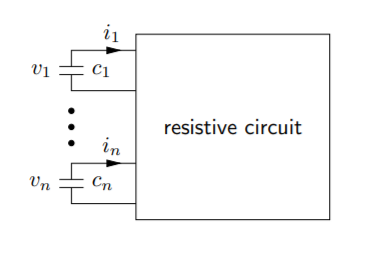
\includegraphics[width=0.5\textwidth]{images/image1.png}}\par}

The circuit is represented by a matrix of conductivities. What kind of structures might be present in a VLSI chip? The materials seeem to imply that they are dense, but since the actual conductivities are based on the design of chips to be modelled. Given a schematic for a VLSI chip, how do you construct a matrix?


{Some other readings}



{\href{https://www.google.com/url?q=https://www.mpi-magdeburg.mpg.de/2917420/lecture1-handout.pdf\&sa=D\&ust=1575490230666000}{https://www.mpi-magdeburg.mpg.de/2917420/lecture1-handout.pdf}}


\begin{itemize}
\tightlist
\item
  {Model reduction is a topic that comes up frequently. The size of the
  VLSI matrix is so massive that it is only feasible to process it when
  it has been simplified}
\item
  It appears to be linear system, but this is not explicitly verified
  in the slides.
\item
  thermic/electro magnetic effects are what can disturb the signal;
  multilayered chips are a problem. How does this come into play 
  when representing the system?
\item
  Existing methods include Pade approximation, rational interpolation, 
  and rational interpolation. How have these examples been constructed?
\end{itemize}

{Problems/questions}

\begin{itemize}
\tightlist
\item
  {I haven't seen a resource that actually verifies that we're modelling
  the effects of a delta signal. The above picture from the stanford
  slides implies it, but only for a toy example}
\item
  {What kind of circuits are represented? Just a network of resistors?
  How do I construct a matrix A such that it represents a realistic VLSI
  system that someone is interested in modelling in modern
  applications?}
\end{itemize}

{}

{Irrelevant things}

\begin{itemize}
\tightlist
\item
  {\href{https://www.google.com/url?q=https://link.springer.com/article/10.1007/BF02471131\&sa=D\&ust=1575490230669000}{https://link.springer.com/article/10.1007/BF02471131}}{~seems
  like it's solving the exact opposite problem, using a VLSI chip to
  model a different dynamical system}
\end{itemize}

{}

{}

{}

{}

{}

{}

\end{document}
